\documentclass{standalone}
\usepackage{graphicx}	
\usepackage{amssymb, amsmath}
\usepackage{color}

\usepackage{tikz}
\usetikzlibrary{intersections, backgrounds}

\definecolor{light}{RGB}{220, 188, 188}
\definecolor{mid}{RGB}{185, 124, 124}
\definecolor{dark}{RGB}{143, 39, 39}
\definecolor{highlight}{RGB}{180, 31, 180}
\definecolor{gray10}{gray}{0.1}
\definecolor{gray20}{gray}{0.2}
\definecolor{gray30}{gray}{0.3}
\definecolor{gray40}{gray}{0.4}
\definecolor{gray60}{gray}{0.6}
\definecolor{gray70}{gray}{0.7}
\definecolor{gray80}{gray}{0.8}
\definecolor{gray90}{gray}{0.9}
\definecolor{gray95}{gray}{0.95}

\newcommand*{\offset}{0.025}

\begin{document}

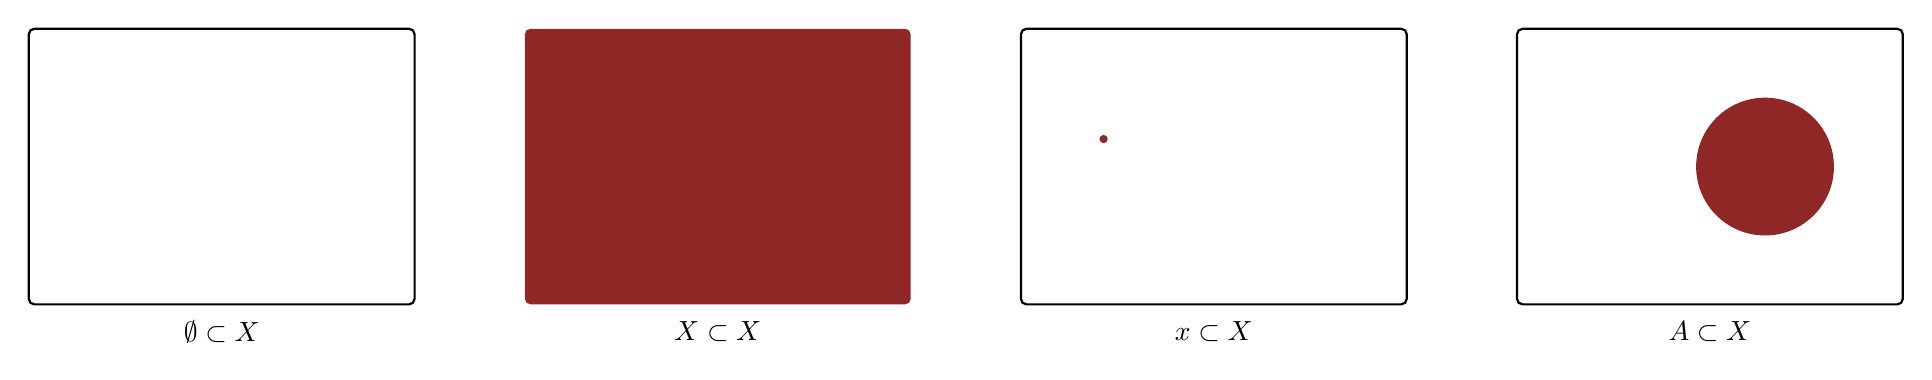
\begin{tikzpicture}[scale=0.35, thick]
  % Empty
  \draw [rounded corners=2pt, color=black] (-2, 0) rectangle +(-14, 10);
  \node at (-9, -1) { $\emptyset \subset X$ };

  % Full
  \fill [rounded corners=2pt, color=dark] (2, 0) rectangle +(14, 10);
  \node at (9, -1) { $X \subset X$ };

  % Point
  \draw [rounded corners=2pt, color=black] (20, 0) rectangle +(14, 10);
  \fill [fill=dark, text=black] (23, 6) circle (0.15);
  \node at (27, -1) { $x \subset X$ };

  % General
  \draw [rounded corners=2pt, color=black] (38, 0) rectangle +(14, 10);
  \node at (45, -1) { $A \subset X$ };  
  \fill [fill=dark, text=white] (47, 5) circle (2.5);
 
  
\end{tikzpicture}

\end{document}  